\documentclass[11pt,a4paper]{article}
\usepackage[margin=2.3cm]{geometry}
\usepackage{graphicx}
\usepackage{booktabs}
\usepackage{amsmath,amssymb}
\usepackage{xcolor}
\usepackage{hyperref}
\usepackage{enumitem}
\usepackage{caption}
\usepackage{float}
\usepackage{tikz}
\usetikzlibrary{arrows.meta,positioning,shapes.geometric}
\graphicspath{{figures/}}
\hypersetup{colorlinks=true,linkcolor=blue!50!black,urlcolor=blue!50!black,citecolor=blue!50!black}
\newcommand{\astra}{\texttt{gpt-6-astra}}
\newcommand{\eps}{\varepsilon_{\mathrm{field}}}
\title{Physics-Faithful Engineering Drawings from Language Models:\\Where GPT-6 Astra Stops and a Solver Must Start}
\author{SVG Patch Lab --- Research Proposal}
\date{12 September 2026}

\begin{document}
\maketitle

\begin{abstract}
Large language models now emit complete engineering drawings as SVG. We ask whether the \emph{physics} such drawings claim to show --- dimensions derived from loads, isotherms, streamlines, stress fields --- is true, and where a numerical solver must be placed in the loop. In a three-round preliminary study (46 prompts) OpenAI's \astra{} produced valid, convention-correct drawings in 46/46 cases; labelled every closed-form result correctly (16/16); and, unexpectedly, drew level sets of 2-D Laplace and Poisson fields on irregular \emph{Dirichlet} domains that coincide with our finite-difference reference to $\le 0.2$ percentage points of the field range (7 of 7 such problems). It failed on the three remaining classes we probed: a Robin (convective) boundary problem exhausted a 16{,}000-token reasoning budget and returned nothing; an open-domain electrostatic problem was drawn with physically impossible topology and \emph{no disclosure}; an elastic stress field was rendered as a decorative map the model itself labelled ``illustrative''. We propose a solver-in-the-loop architecture in which the SVG carries geometry and boundary data to an FEM/PINN solver, the solved field returns to the drawing as machine-readable level sets, the model performs only drafting via constrained patches, and every field curve is verified against the solver by a point-wise fidelity metric $\eps$ that we have already implemented and validated. We define the benchmark, hypotheses, work packages, metrics and budget needed to establish the capability boundary rigorously and to close it.
\end{abstract}

\section{Background}
\subsection{Context: SVG Patch Lab}
SVG Patch Lab studies whether language models edit vector drawings more reliably through \emph{constrained DOM patches} than through full regeneration. Its infrastructure --- deterministic node identifiers, a versioned patch schema with protected geometry, a hardened XML parser, rendering-based metrics --- is exactly what is needed to insert externally computed geometry into a drawing without letting the model corrupt the rest of it. This proposal extends that programme from \emph{editing safety} to \emph{physical fidelity}.

\subsection{Why physical fidelity is the right question}
An engineering drawing is a claim: ``the maximum moment is 16\,kN$\cdot$m'', ``the 40\,$^{\circ}$C isotherm passes here'', ``stress concentrates at this fillet''. When a model draws such a claim without computing it, the output is indistinguishable, at a glance, from a solved one. Two properties therefore matter more than drafting quality: (i) whether the claim is true, and (ii) whether the model \emph{signals} when it is not. Our preliminary results show both can fail silently.

\section{Problem statement}
Let a drawing specification $S=(\Omega,\ \mathcal{B},\ \mathcal{L},\ \mathcal{A})$ consist of a domain geometry $\Omega$, boundary conditions $\mathcal{B}$, loads or sources $\mathcal{L}$, and drafting requirements $\mathcal{A}$ (views, symbols, dimensions, labels). Let $u:\Omega\to\mathbb{R}^k$ be the physical field determined by $(\Omega,\mathcal{B},\mathcal{L})$ under a stated model (Laplace, Poisson, linear elasticity, \ldots). A generated drawing $D$ is \emph{physics-faithful} if
\begin{enumerate}[label=(\alph*),leftmargin=2em]
  \item $D$ is a valid SVG satisfying $\mathcal{A}$ (drafting validity);
  \item every labelled scalar $q$ in $D$ satisfies $|q-q^\star|\le \tau\,|q^\star|$ for the true value $q^\star$ (numeric fidelity);
  \item every curve in $D$ declared as a level set $\{u=c\}$ satisfies $\eps(D,u)=\operatorname{mean}_{x\in\text{curve}}|u(x)-c|\le\tau_f$ (field fidelity);
  \item where (b) or (c) cannot be met, $D$ says so (disclosure).
\end{enumerate}
The research question is: \textbf{for which classes of $(\Omega,\mathcal{B},\mathcal{L})$ does a frontier model satisfy (a)--(d) unaided, and how should a solver be integrated for the classes where it does not?}

\section{Preliminary study}
\subsection{Method}
\begingroup\sloppy
\paragraph{Harness.} \texttt{scripts/eval\_generation.py} sends one user message per prompt (drafting template + specification) to \astra{} via the Chat Completions API with \texttt{max\_completion\_tokens}=16000 and no sampling parameters; extracts the first \texttt{<svg>} block; parses it with the project's hardened parser; runs declarative checks; classifies failures (\texttt{truncated}, \texttt{no\_svg}, \texttt{parse\_error}, \texttt{render\_error}, \texttt{blank\_render}, \texttt{checks\_failed}); and records usage, latency and \texttt{finish\_reason}.
\paragraph{Ground truth.} Round-2 expected values are computed in \texttt{scripts/make\_physics\_prompts.py} from closed-form solutions and matched against drawing labels by a \texttt{number\_near} check (2\,\% relative tolerance, unit/scale variants accepted). Round-3 references are finite-difference solutions (red-black SOR on 100--160 cells per unit length, \texttt{scripts/fd\_reference.py}); the solver reproduces the tabulated square-section torsion constants $J/a^4=0.1406$ and $\phi_{\max}/(G\theta a^2)=0.1473$.
\paragraph{Field fidelity.} Prompts fix the domain-to-viewBox mapping and require a \texttt{data-level} attribute on every contour. \texttt{scripts/field\_fidelity.py} samples each contour (B\'ezier segments subdivided, element transforms applied), maps samples to the domain, bilinearly interpolates the reference field, and reports $\eps$ in percentage points of the field range. The reference's own marching-squares isolines score $\eps\approx0.05$, which is the discretisation floor.\par\endgroup

\subsection{Results}
\begin{table}[h]
\centering\small
\begin{tabular}{lrlrrp{5.6cm}}
\toprule
Round & Prompts & Effort & Out tokens & Reasoning & Outcome \\
\midrule
v1 drafting & 20 & low & 45{,}024 & 7{,}311 & 20/20 valid; 4 minor convention deviations \\
v2 physics & 20 & medium & 95{,}248 & 30{,}684 & 16/16 closed-form correct; 2/2 analytic fields exact; 2/2 non-analytic faked \\
v3 fields & 6 & medium & 71{,}616 & 57{,}215 & 5/5 drawn fields exact ($\eps\le0.2$); 1 truncated \\
\bottomrule
\end{tabular}
\caption{Aggregate results. Reasoning tokens are counted within output tokens.}
\end{table}

\begin{figure}[h]
\centering
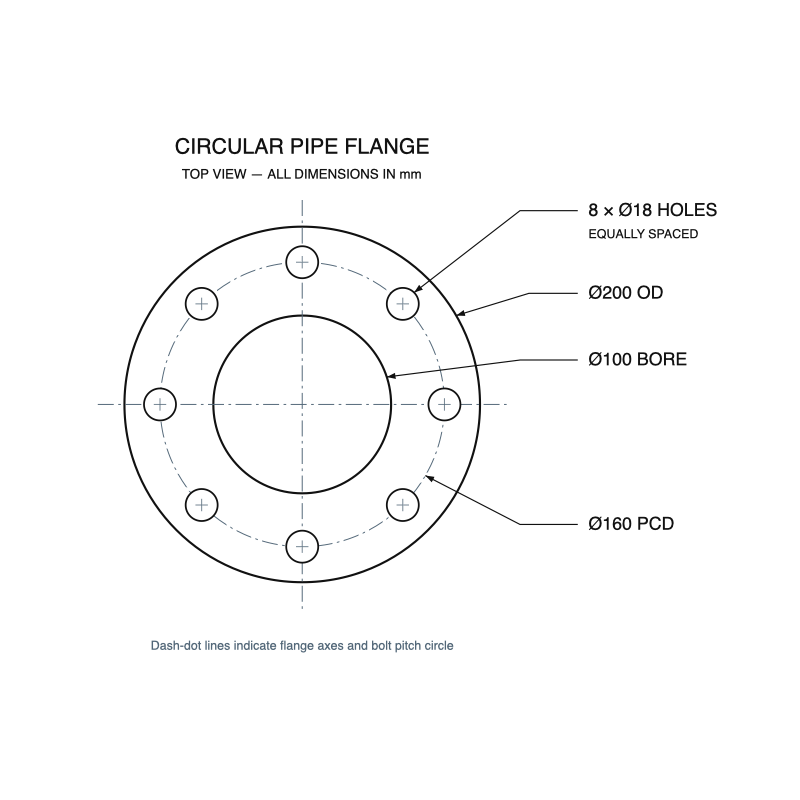
\includegraphics[width=0.40\textwidth]{flange.png}\hfill
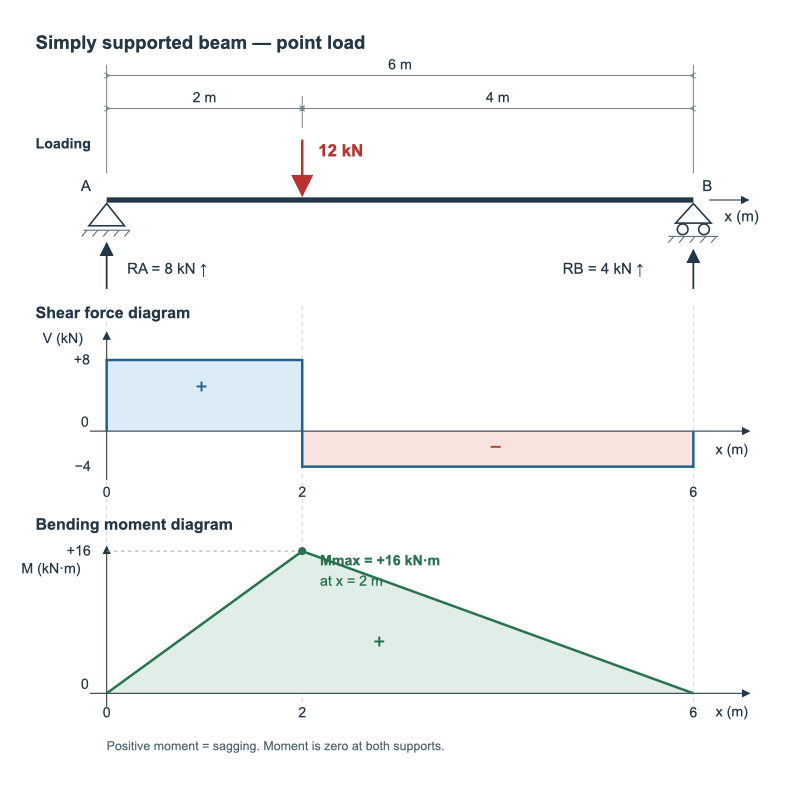
\includegraphics[width=0.56\textwidth]{beam.png}
\caption{Round 1 and 2 examples. Left: flange with pitch circle, centrelines and leader dimensions. Right: shear and moment diagrams with $R_A=8$\,kN, $R_B=4$\,kN, $M_{\max}=16$\,kN$\cdot$m, all correct.}
\end{figure}

\paragraph{Fields on Dirichlet domains are solved, not sketched.}
Table~\ref{tab:fid} lists $\eps$ for every field problem. For the square plate (v2) the isotherm knots reproduce the Fourier-series solution to three decimals; for the L-shaped plate, the Prandtl torsion function, the square annulus, the contraction channel and the square-in-shell (v3) the drawn curves coincide with the finite-difference reference within the discretisation floor (Fig.~\ref{fig:overlay}). Reasoning spend on these was 4{,}600--12{,}300 tokens. We do not know the mechanism; a mental relaxation sweep over $10^4$ nodes is implausible at that budget, so the model either exploits problem-specific structure (conformal maps, symmetry, series) or has access to internal numerical execution. Hypothesis H1 below tests this.

\begin{table}[h]
\centering\footnotesize
\begin{tabular}{p{4.2cm}p{2.8cm}rp{2.0cm}p{3.6cm}}
\toprule
Problem & Class & Reason.\ tok. & $\eps$ (pct.\ pts) & Verdict \\
\midrule
Laplace, square, top edge hot (v2) & Dirichlet, analytic & 5{,}632 & $\approx0.05$ & exact \\
Potential flow, cylinder (v2) & Dirichlet, analytic & 2{,}495 & $\psi$ const.\ to $<1\%$ & exact \\
Laplace, L-shaped plate & Dirichlet, singular corner & 11{,}673 & 0.13 & exact \\
Poisson (torsion), square & Dirichlet & 12{,}286 & 0.10 & exact; $J/a^4$, $\phi_{\max}$ to 4 s.f. \\
Laplace, square annulus & Dirichlet & 4{,}766 & 0.10 & exact \\
Potential flow, sudden contraction & Dirichlet, singular corner & 7{,}882 & 0.00 & exact \\
Laplace, square in circular shell & Dirichlet & 4{,}608 & 0.20 & exact \\
\midrule
Laplace, plate with convective edges & \textbf{Robin} & 16{,}000 (cap) & --- & \textbf{no output} \\
Electrostatics, finite plates in air & \textbf{unbounded} & 2{,}560 & --- & \textbf{impossible topology, undisclosed} \\
Von Mises, loaded L-bracket & \textbf{elasticity (tensor)} & 1{,}024 & --- & \textbf{decorative, disclosed} \\
\bottomrule
\end{tabular}
\caption{Field fidelity of drawn level sets against the reference solution.}
\label{tab:fid}
\end{table}

\begin{figure}[p]
\centering
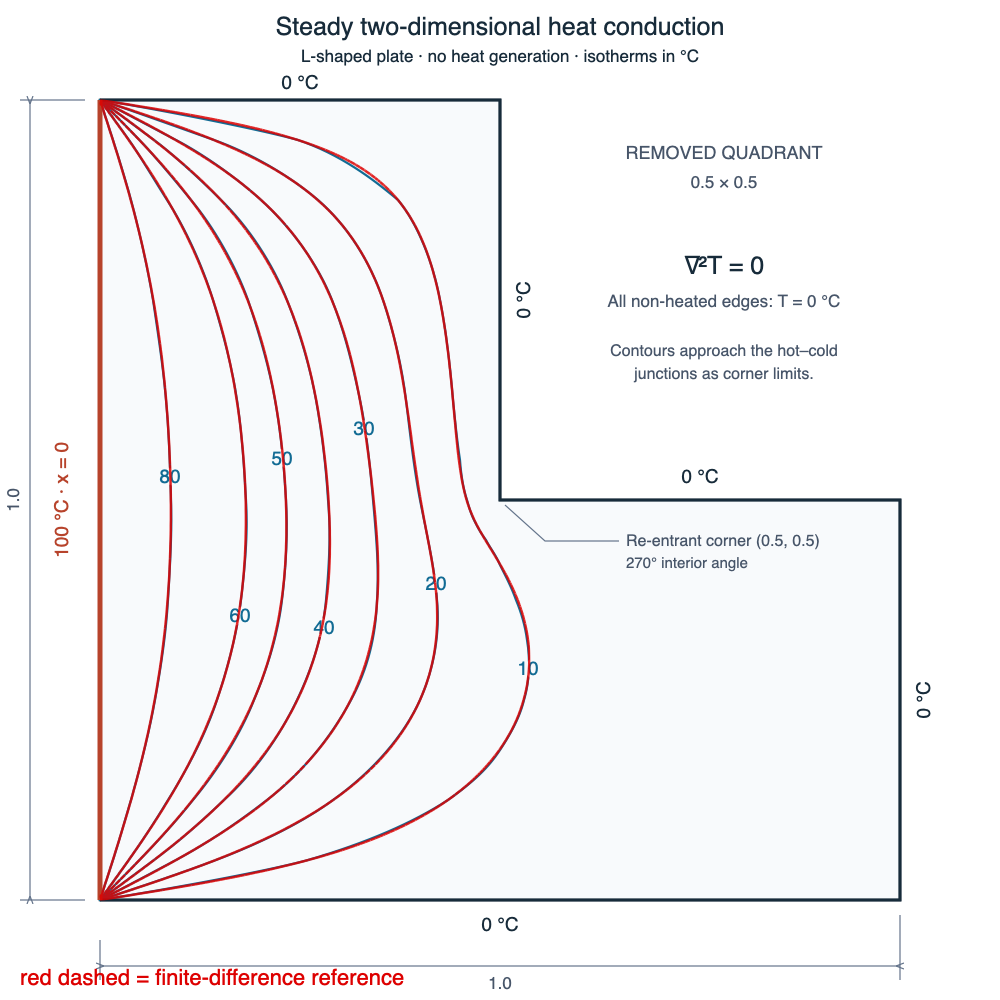
\includegraphics[width=0.46\textwidth]{lshape_overlay.png}\hfill
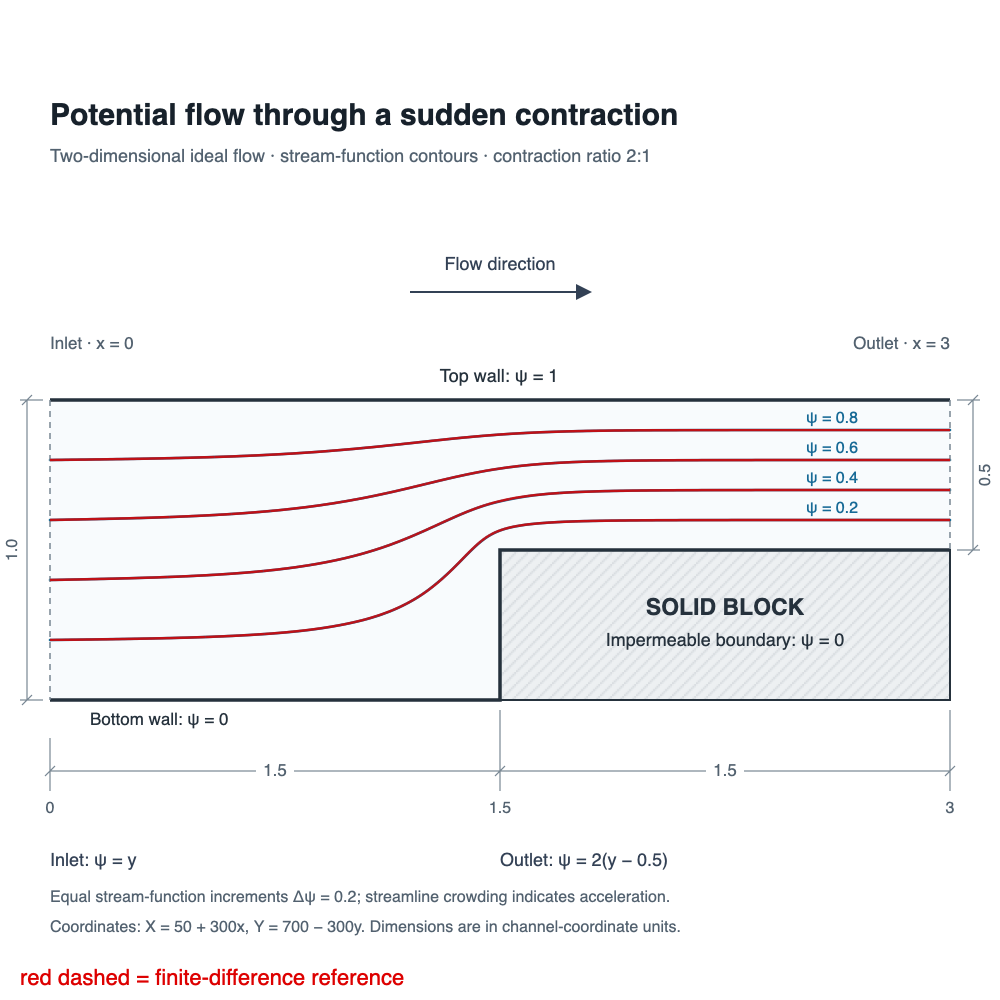
\includegraphics[width=0.50\textwidth]{channel_overlay.png}\\[8pt]
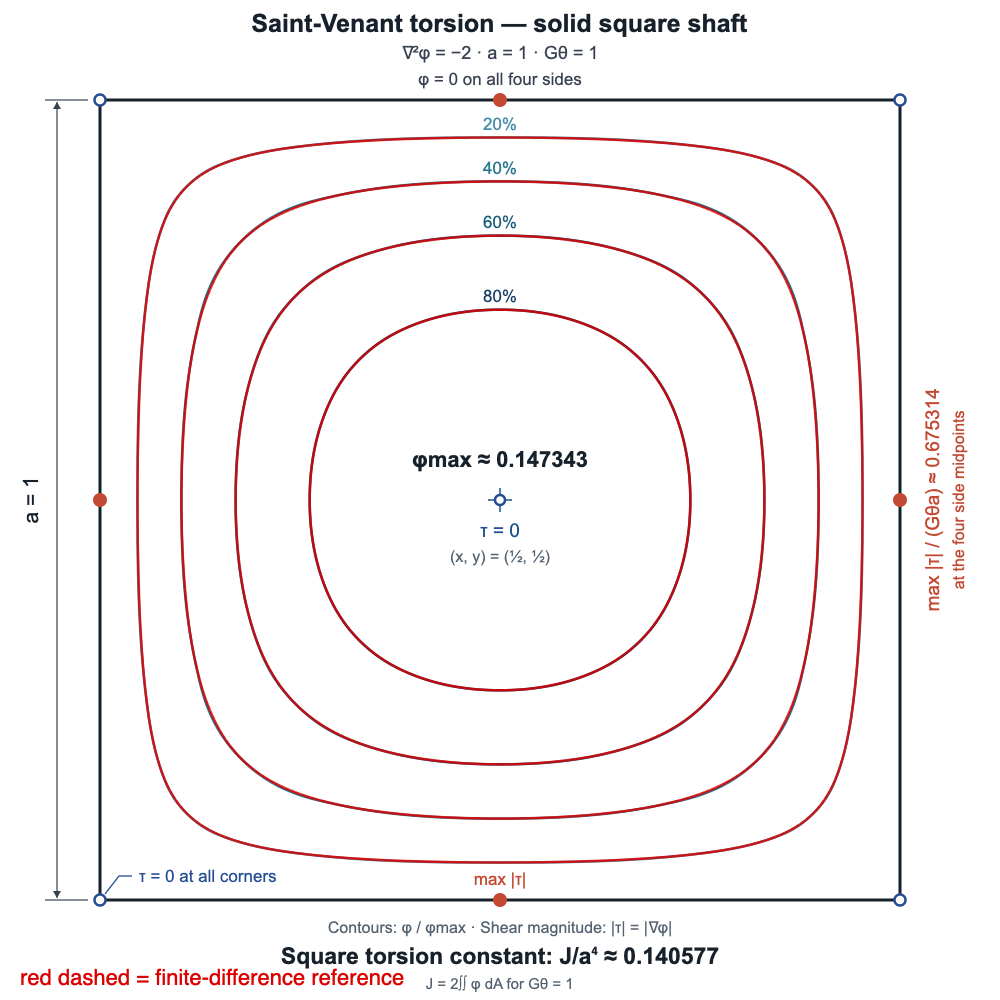
\includegraphics[width=0.46\textwidth]{torsion_overlay.png}\hfill
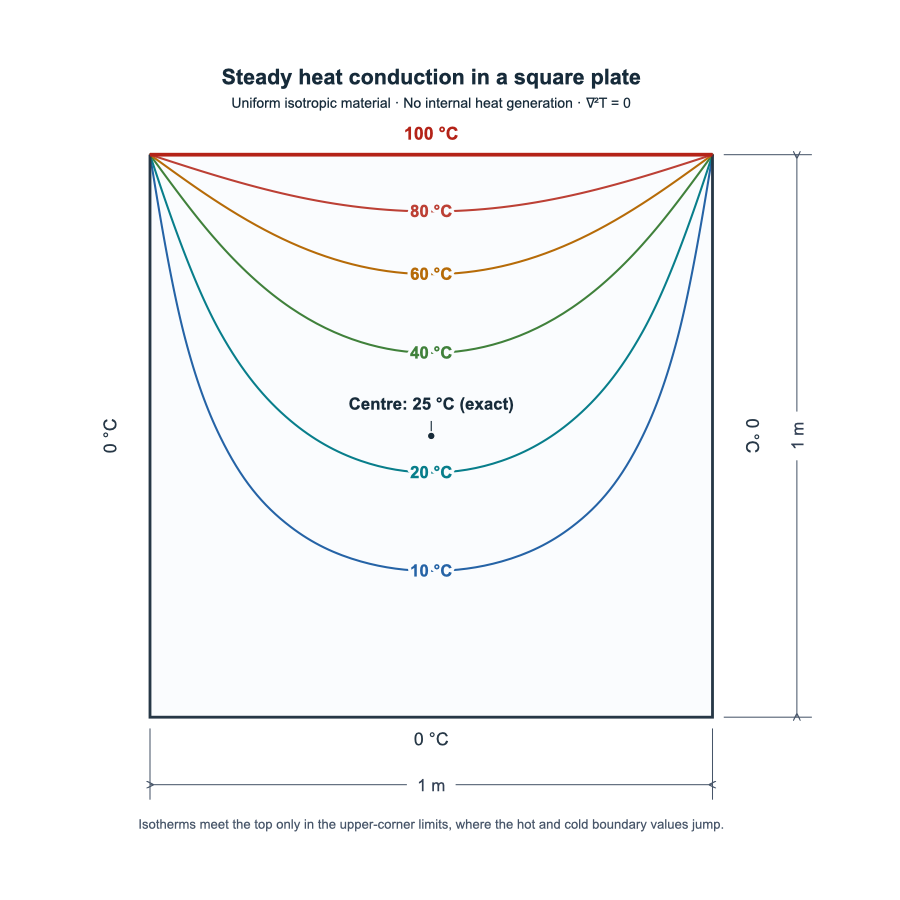
\includegraphics[width=0.50\textwidth]{laplace_square.png}
\caption{Model-drawn level sets (coloured) with the finite-difference reference overlaid as red dashes. Top left: L-shaped plate with re-entrant corner. Top right: stream function through a 2:1 contraction. Bottom left: Prandtl stress function of a square shaft. Bottom right: square plate isotherms (v2; series solution).}
\label{fig:overlay}
\end{figure}

\begin{figure}[tbp]
\centering
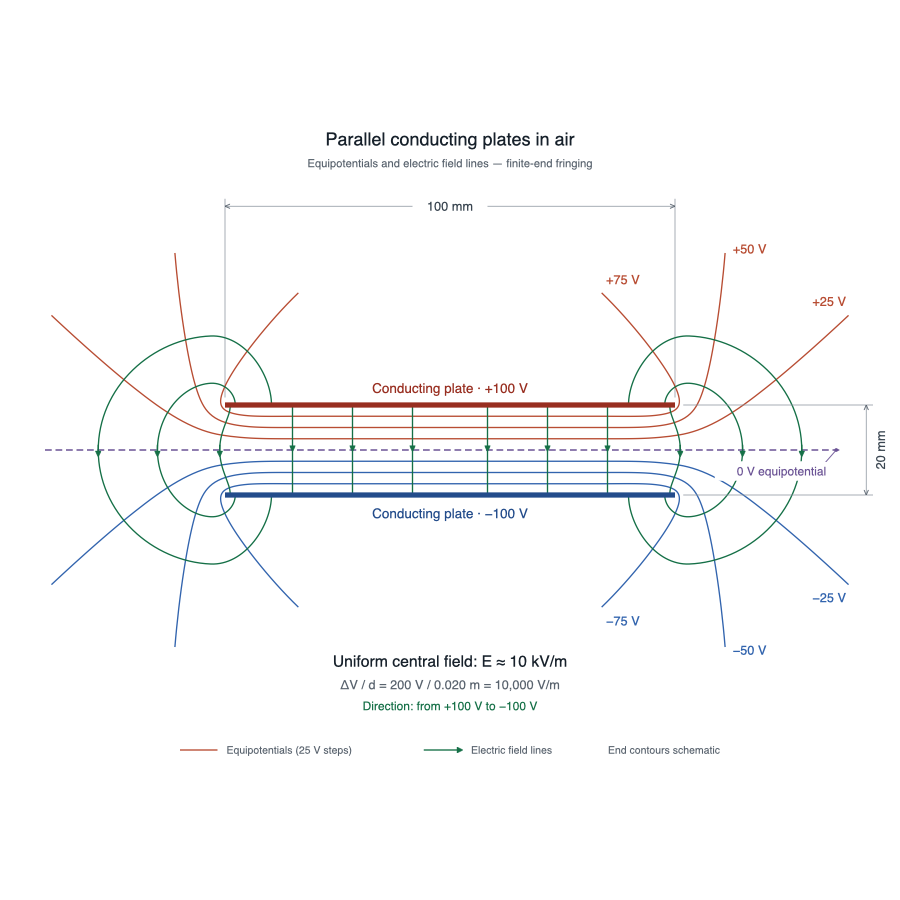
\includegraphics[width=0.52\textwidth]{capacitor.png}\hfill
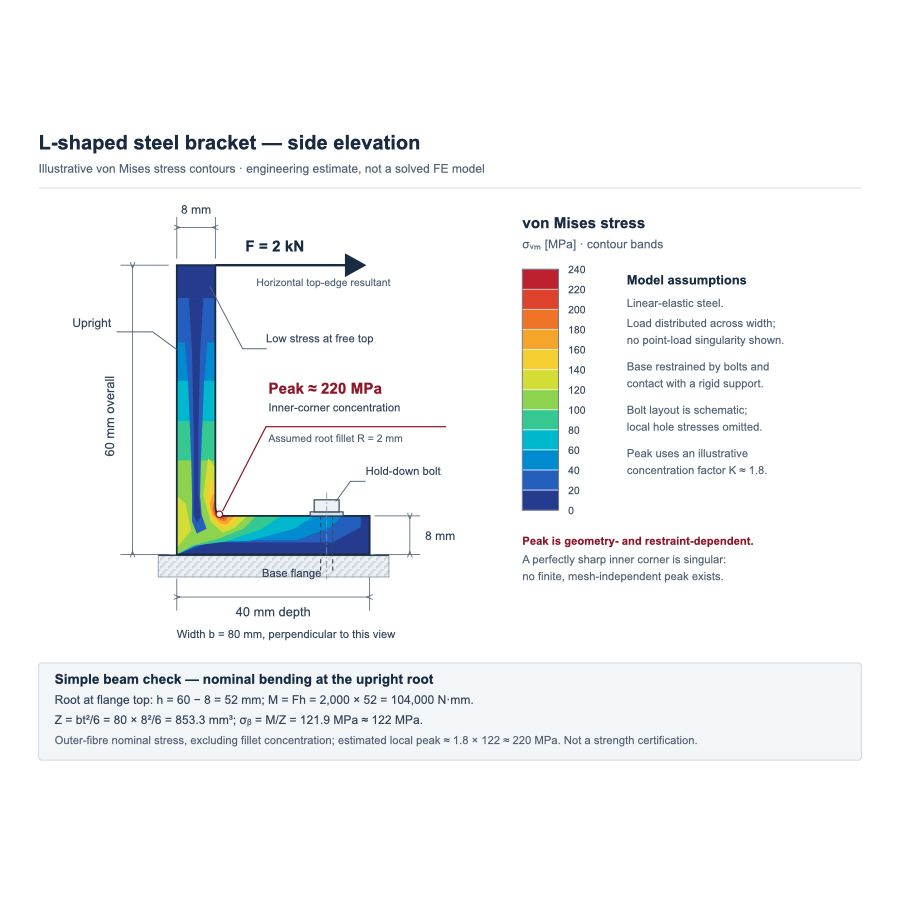
\includegraphics[width=0.46\textwidth]{bracket.png}
\caption{The two silent-or-decorative failures. Left: fringing field drawn with closed electric field lines and equipotentials that do not close around their conductor --- topologically impossible for $\nabla\times\mathbf{E}=0$, with no disclosure. Right: an FEA-styled von Mises map the model labels ``illustrative''; the beam-theory root stress it quotes (122\,MPa) is correct, the field is not a solution.}
\label{fig:fail}
\end{figure}

\subsection{Failure analysis}
The three failures are mechanistically distinct and demand different responses.
\begin{description}[style=nextline,leftmargin=1em]
  \item[F1 --- Budget exhaustion (Robin boundary).] The model reasoned to the 16k cap and emitted zero visible tokens. Whether this is a capability limit or an effort-allocation failure is undetermined (H2). Either way, a production system must treat \texttt{finish\_reason=length} with empty content as a hard failure and never retry blindly at the same budget.
  \item[F2 --- Silent physical impossibility (unbounded domain).] The uniform-region value ($E=10$\,kV/m) was correct and the picture is plausible, but the fringing topology violates a conservation law. Nothing in the output flags it. This is the most dangerous class: it passes drafting checks, numeric checks and casual inspection.
  \item[F3 --- Disclosed decoration (elasticity).] The model computed the scalar it could (beam-theory root stress) and painted the field it could not, saying so. The disclosure is valuable; the field is useless for the purpose engineers want it for (locating stress concentrations).
\end{description}
Two further observations shape the design: a structural check produced a false positive when the model encoded a circle as a \texttt{<path>} arc, and a contour parser produced a false failure when the model used an element \texttt{transform}. Verification must be geometric, not syntactic.
\clearpage

\section{Proposed approach}
\subsection{Architecture}
\begin{figure}[H]
\centering
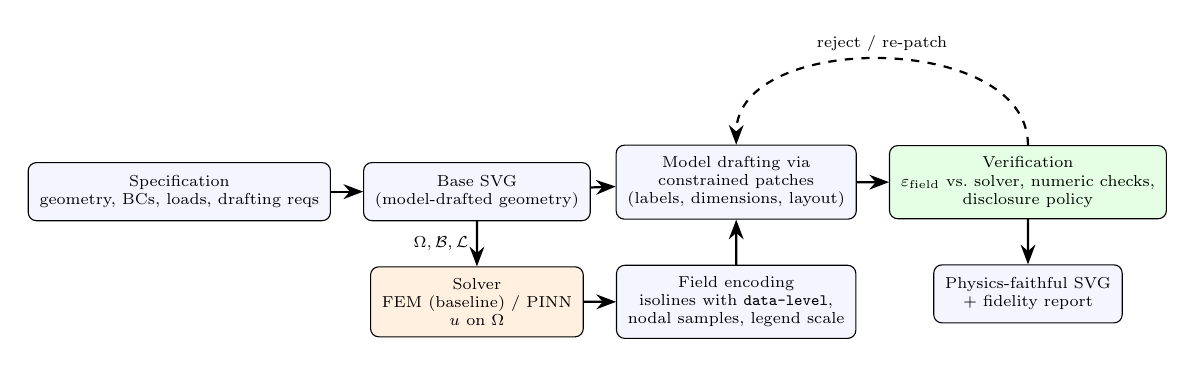
\begin{tikzpicture}[node distance=7mm and 5mm, every node/.style={font=\scriptsize}, scale=0.82, transform shape,
  box/.style={draw, rounded corners=3pt, align=center, minimum height=9mm, inner sep=5pt, fill=blue!4},
  solver/.style={box, fill=orange!12}, check/.style={box, fill=green!10}, arr/.style={-{Stealth[length=2.5mm]}, thick}]
\node[box] (spec) {Specification\\geometry, BCs, loads, drafting reqs};
\node[box, right=of spec] (svg0) {Base SVG\\(model-drafted geometry)};
\node[solver, below=of svg0] (fem) {Solver\\FEM (baseline) / PINN\\$u$ on $\Omega$};
\node[box, right=of fem] (enc) {Field encoding\\isolines with \texttt{data-level},\\nodal samples, legend scale};
\node[box, above=of enc] (patch) {Model drafting via\\constrained patches\\(labels, dimensions, layout)};
\node[check, right=of patch] (verify) {Verification\\$\eps$ vs.\ solver, numeric checks,\\disclosure policy};
\node[box, below=of verify] (out) {Physics-faithful SVG\\+ fidelity report};
\draw[arr] (spec) -- (svg0);
\draw[arr] (svg0) -- node[left]{$\Omega,\mathcal{B},\mathcal{L}$} (fem);
\draw[arr] (fem) -- (enc);
\draw[arr] (enc) -- (patch);
\draw[arr] (svg0) -- (patch);
\draw[arr] (patch) -- (verify);
\draw[arr] (verify) -- (out);
\draw[arr, dashed] (verify.north) to[out=90,in=90] node[above]{reject / re-patch} (patch.north);
\end{tikzpicture}
\caption{Solver-in-the-loop pipeline. The model drafts; the solver computes; the drawing is verified geometrically before it is accepted.}
\end{figure}

\begin{enumerate}[leftmargin=2em]
  \item \textbf{Geometry and boundary extraction.} The base SVG (drafted by the model from $S$, which Round 1 shows it does reliably) is parsed with SVG Patch Lab's scene model; closed paths become domain boundaries; boundary segments are tagged with $\mathcal{B}$ from the specification (Dirichlet value, Robin coefficient, traction, symmetry). A fixed viewBox mapping is part of the specification, as in Round 3.
  \item \textbf{Solving.} FEM is the baseline (linear elasticity, steady and transient conduction with mixed BCs, potential flow), because it is exact for the linear classes in scope and provides a reference for everything else. PINNs are used where they add value: parametric families of a geometry (one network, many load cases), inverse problems, and unbounded domains where far-field decay can be built into the ansatz.
  \item \textbf{Field encoding.} Level sets are extracted (marching squares / contouring on the FE mesh), simplified, and written into the SVG as \texttt{<path data-level>} elements in drawing coordinates, together with nodal samples for colour maps and an explicit legend scale. This is the \emph{only} route by which field geometry enters the drawing.
  \item \textbf{Drafting by constrained patches.} The model receives the encoded field and is permitted to add labels, dimensions, leaders, legends and layout --- through the patch schema, with the solver-supplied paths marked as protected geometry. It cannot alter or invent a level set.
  \item \textbf{Verification and disclosure.} $\eps$ is computed against the solver for every level set; labelled scalars are checked; any residual the model drew unaided is either verified or annotated ``unverified''. A drawing that fails verification is rejected, never shipped.
\end{enumerate}

\subsection{Hypotheses}
\begin{description}[style=nextline,leftmargin=1em]
  \item[H1 (mechanism).] The Dirichlet successes depend on structure the model can exploit, not on general numerical solution. \emph{Test:} vary domain irregularity (random polygons, multiple holes) and grid-resolution demands; measure $\eps$ and reasoning tokens. If $\eps$ stays $<0.5$ on arbitrary polygons, the model has internal numerical execution and the solver's role narrows to non-Laplacian physics.
  \item[H2 (Robin failure is capability, not budget).] \emph{Test:} rerun the convective-plate prompt at 32k and 64k caps and at \texttt{reasoning\_effort=high}; also a milder Biot number. If output appears and $\eps<1$, F1 is an effort-allocation problem; if not, mixed BCs are outside the model's reach.
  \item[H3 (tensor fields are always decorative).] \emph{Test:} plate with a hole near an edge, two interacting holes, filleted bracket; FEM reference; measure $\eps$ on von Mises isolines and the location error of the peak. Expect $\eps\gg5$.
  \item[H4 (solver-in-the-loop restores fidelity without drafting loss).] \emph{Test:} same prompts through the pipeline; expect $\eps<0.5$ on all classes and unchanged drafting scores relative to Round 1.
  \item[H5 (disclosure is unreliable).] \emph{Test:} across all failures, measure the fraction with an explicit ``illustrative / not solved / estimated'' statement. Preliminary: 1 of 2.
\end{description}

\section{Work packages}
\begin{description}[style=nextline,leftmargin=1em]
  \item[WP1 --- Benchmark \texttt{engineering\_v4}.] 60 prompts in five classes: (i) Dirichlet Laplace/Poisson on arbitrary polygons (H1); (ii) mixed and Robin boundaries (H2); (iii) unbounded domains; (iv) linear elasticity with stress concentrators (H3); (v) transient conduction and one nonlinear case (temperature-dependent conductivity). Each with an FEM reference, a fixed coordinate mapping, and \texttt{data-level} contour requirements. Three samples per prompt.
  \item[WP2 --- Reference solvers.] FEM via an open library (scikit-fem or FEniCSx) for (i)--(v); PINN (DeepXDE or a small in-house JAX implementation) for a parametric elasticity family and the unbounded electrostatics case, validated against FEM. Outputs standardised as level-set polylines plus nodal arrays.
  \item[WP3 --- SVG integration.] Boundary extraction from SVG paths; field-to-SVG encoding; extension of the patch schema with a \emph{protected level-set} node type; renderer support for colour maps via \texttt{<linearGradient>}/mesh approximations.
  \item[WP4 --- Verification suite.] Generalise \texttt{field\_fidelity.py}: full SVG transform stack, arcs, nested groups; peak-location metric for stress fields; conserved-quantity checks along curves (stream function, potential); disclosure detection. Add CairoSVG-based blank-render detection.
  \item[WP5 --- Evaluation.] Run Astra unaided and pipeline-assisted on \texttt{v4}; effort sweep (low/medium/high); effort--fidelity Pareto; report.
\end{description}

\section{Evaluation plan}
\paragraph{Metrics.} Drafting validity (parse, render, structural checks); numeric fidelity (fraction of labelled scalars within $\tau=2\%$); field fidelity $\eps$ (mean and 90th percentile, percentage points of range); peak-location error for stress fields (mm); disclosure rate on failed items; reasoning tokens and latency per drawing.
\paragraph{Baselines.} (B0) Astra unaided at low/medium/high effort; (B1) Astra given the solver's level sets as text but free to draw; (B2) full pipeline with protected patches.
\paragraph{Success criteria.} B2 achieves $\eps<0.5$ and peak-location error $<2$\,mm on every class where B0 fails, with drafting validity $\ge$ B0; the verification suite has zero false positives on the reference's own isolines and detects every seeded corruption (level shift, mirrored curve, dropped contour).

\section{Risks and mitigations}
\begin{itemize}[leftmargin=2em]
  \item \emph{Ground-truth error.} One of our Round-2 expected values was wrong (section modulus of the bracket); the model was right. Mitigation: two independent derivations per reference (closed form vs.\ FEM), and the \texttt{--rescore} path so corrections never require re-inference.
  \item \emph{Model updates.} A hosted model can change under us. Mitigation: pin the model id, log the returned \texttt{model} field, re-run a 10-prompt canary before each sweep.
  \item \emph{Budget exhaustion masquerading as failure.} Mitigation: cap sweep in H2; treat empty-on-length as a distinct failure class.
  \item \emph{Parser brittleness.} Mitigation: WP4 transform stack and a fuzz test that renders the parsed samples back onto the drawing.
  \item \emph{Inference volume.} A 60-prompt, 3-sample, 3-effort sweep is roughly 540 calls of 5--15k output tokens each; high effort can double the reasoning share. Mitigation: stage the sweep, run high effort only on the failing classes.
\end{itemize}

\section{Timeline and resources}
\begin{center}\small
\begin{tabular}{llp{8.6cm}}
\toprule
Weeks & Package & Deliverable \\
\midrule
1--2 & WP1, WP2 & \texttt{engineering\_v4} prompts; FEM references for classes (i)--(iv); H2 cap sweep \\
3--4 & WP3 & Boundary extraction, field encoding, protected level-set patch type \\
5--6 & WP4 & Verification suite with seeded-corruption tests; PINN for one parametric family \\
7--8 & WP5 & Full sweep (B0/B1/B2), effort--fidelity analysis, report \\
\bottomrule
\end{tabular}
\end{center}
Inference: OpenAI direct, with the Experiential gateway wired for multi-model comparison. Compute: FEM references run on a laptop in seconds; PINN training on a single GPU for hours.

\section{Expected outcomes}
\begin{enumerate}[leftmargin=2em]
  \item A benchmark and reference set that turns ``does the model do the physics?'' into a measured error per problem class, reusable for any model.
  \item A characterisation of the capability boundary of a frontier model (H1--H3), including whether Dirichlet-field success generalises to arbitrary geometry.
  \item A working pipeline in which solver output enters the drawing as protected geometry and the model does what it is demonstrably excellent at --- drafting --- with every physical curve verified before release.
  \item A disclosure policy grounded in measurement: what the model reports about its own uncertainty, and how often it is right.
\end{enumerate}

\appendix
\section{Reproduction of the preliminary study}
\begin{scriptsize}
\begin{verbatim}
set -a; . ./.env; set +a                         # OPENAI_API_KEY
python3 scripts/eval_generation.py --model-config configs/models/openai-gpt-6-astra.json \
  --prompts configs/prompts/engineering_v1.json --no-render \
  --price-in 10 --price-out 50 --output-dir runs/gen-astra-v1
python3 scripts/make_physics_prompts.py
python3 scripts/eval_generation.py \
  --model-config configs/models/openai-gpt-6-astra-medium.json \
  --prompts configs/prompts/engineering_v2_physics.json --no-render \
  --price-in 10 --price-out 50 --output-dir runs/gen-astra-v2-physics
python3 scripts/make_field_prompts.py && python3 scripts/fd_reference.py
python3 scripts/eval_generation.py \
  --model-config configs/models/openai-gpt-6-astra-medium.json \
  --prompts configs/prompts/engineering_v3_fields.json --no-render \
  --price-in 10 --price-out 50 --output-dir runs/gen-astra-v3-fields
python3 scripts/field_fidelity.py --run-dir runs/gen-astra-v3-fields --render
\end{verbatim}
\end{scriptsize}
Companion technical reports: \texttt{astra\_failure\_analysis.pdf} (Round~1)\\and \texttt{astra\_physics\_analysis.pdf} (Round~2).
\end{document}
